\documentclass[]{article}
\usepackage{lmodern}
\usepackage{amssymb,amsmath}
\usepackage{ifxetex,ifluatex}
\usepackage{fixltx2e} % provides \textsubscript
\ifnum 0\ifxetex 1\fi\ifluatex 1\fi=0 % if pdftex
  \usepackage[T1]{fontenc}
  \usepackage[utf8]{inputenc}
\else % if luatex or xelatex
  \ifxetex
    \usepackage{mathspec}
  \else
    \usepackage{fontspec}
  \fi
  \defaultfontfeatures{Ligatures=TeX,Scale=MatchLowercase}
\fi
% use upquote if available, for straight quotes in verbatim environments
\IfFileExists{upquote.sty}{\usepackage{upquote}}{}
% use microtype if available
\IfFileExists{microtype.sty}{%
\usepackage{microtype}
\UseMicrotypeSet[protrusion]{basicmath} % disable protrusion for tt fonts
}{}
\usepackage[margin=1in]{geometry}
\usepackage{hyperref}
\hypersetup{unicode=true,
            pdftitle={Generalized Linear Models - Count Response},
            pdfborder={0 0 0},
            breaklinks=true}
\urlstyle{same}  % don't use monospace font for urls
\usepackage{color}
\usepackage{fancyvrb}
\newcommand{\VerbBar}{|}
\newcommand{\VERB}{\Verb[commandchars=\\\{\}]}
\DefineVerbatimEnvironment{Highlighting}{Verbatim}{commandchars=\\\{\}}
% Add ',fontsize=\small' for more characters per line
\usepackage{framed}
\definecolor{shadecolor}{RGB}{248,248,248}
\newenvironment{Shaded}{\begin{snugshade}}{\end{snugshade}}
\newcommand{\AlertTok}[1]{\textcolor[rgb]{0.94,0.16,0.16}{#1}}
\newcommand{\AnnotationTok}[1]{\textcolor[rgb]{0.56,0.35,0.01}{\textbf{\textit{#1}}}}
\newcommand{\AttributeTok}[1]{\textcolor[rgb]{0.77,0.63,0.00}{#1}}
\newcommand{\BaseNTok}[1]{\textcolor[rgb]{0.00,0.00,0.81}{#1}}
\newcommand{\BuiltInTok}[1]{#1}
\newcommand{\CharTok}[1]{\textcolor[rgb]{0.31,0.60,0.02}{#1}}
\newcommand{\CommentTok}[1]{\textcolor[rgb]{0.56,0.35,0.01}{\textit{#1}}}
\newcommand{\CommentVarTok}[1]{\textcolor[rgb]{0.56,0.35,0.01}{\textbf{\textit{#1}}}}
\newcommand{\ConstantTok}[1]{\textcolor[rgb]{0.00,0.00,0.00}{#1}}
\newcommand{\ControlFlowTok}[1]{\textcolor[rgb]{0.13,0.29,0.53}{\textbf{#1}}}
\newcommand{\DataTypeTok}[1]{\textcolor[rgb]{0.13,0.29,0.53}{#1}}
\newcommand{\DecValTok}[1]{\textcolor[rgb]{0.00,0.00,0.81}{#1}}
\newcommand{\DocumentationTok}[1]{\textcolor[rgb]{0.56,0.35,0.01}{\textbf{\textit{#1}}}}
\newcommand{\ErrorTok}[1]{\textcolor[rgb]{0.64,0.00,0.00}{\textbf{#1}}}
\newcommand{\ExtensionTok}[1]{#1}
\newcommand{\FloatTok}[1]{\textcolor[rgb]{0.00,0.00,0.81}{#1}}
\newcommand{\FunctionTok}[1]{\textcolor[rgb]{0.00,0.00,0.00}{#1}}
\newcommand{\ImportTok}[1]{#1}
\newcommand{\InformationTok}[1]{\textcolor[rgb]{0.56,0.35,0.01}{\textbf{\textit{#1}}}}
\newcommand{\KeywordTok}[1]{\textcolor[rgb]{0.13,0.29,0.53}{\textbf{#1}}}
\newcommand{\NormalTok}[1]{#1}
\newcommand{\OperatorTok}[1]{\textcolor[rgb]{0.81,0.36,0.00}{\textbf{#1}}}
\newcommand{\OtherTok}[1]{\textcolor[rgb]{0.56,0.35,0.01}{#1}}
\newcommand{\PreprocessorTok}[1]{\textcolor[rgb]{0.56,0.35,0.01}{\textit{#1}}}
\newcommand{\RegionMarkerTok}[1]{#1}
\newcommand{\SpecialCharTok}[1]{\textcolor[rgb]{0.00,0.00,0.00}{#1}}
\newcommand{\SpecialStringTok}[1]{\textcolor[rgb]{0.31,0.60,0.02}{#1}}
\newcommand{\StringTok}[1]{\textcolor[rgb]{0.31,0.60,0.02}{#1}}
\newcommand{\VariableTok}[1]{\textcolor[rgb]{0.00,0.00,0.00}{#1}}
\newcommand{\VerbatimStringTok}[1]{\textcolor[rgb]{0.31,0.60,0.02}{#1}}
\newcommand{\WarningTok}[1]{\textcolor[rgb]{0.56,0.35,0.01}{\textbf{\textit{#1}}}}
\usepackage{graphicx,grffile}
\makeatletter
\def\maxwidth{\ifdim\Gin@nat@width>\linewidth\linewidth\else\Gin@nat@width\fi}
\def\maxheight{\ifdim\Gin@nat@height>\textheight\textheight\else\Gin@nat@height\fi}
\makeatother
% Scale images if necessary, so that they will not overflow the page
% margins by default, and it is still possible to overwrite the defaults
% using explicit options in \includegraphics[width, height, ...]{}
\setkeys{Gin}{width=\maxwidth,height=\maxheight,keepaspectratio}
\IfFileExists{parskip.sty}{%
\usepackage{parskip}
}{% else
\setlength{\parindent}{0pt}
\setlength{\parskip}{6pt plus 2pt minus 1pt}
}
\setlength{\emergencystretch}{3em}  % prevent overfull lines
\providecommand{\tightlist}{%
  \setlength{\itemsep}{0pt}\setlength{\parskip}{0pt}}
\setcounter{secnumdepth}{0}
% Redefines (sub)paragraphs to behave more like sections
\ifx\paragraph\undefined\else
\let\oldparagraph\paragraph
\renewcommand{\paragraph}[1]{\oldparagraph{#1}\mbox{}}
\fi
\ifx\subparagraph\undefined\else
\let\oldsubparagraph\subparagraph
\renewcommand{\subparagraph}[1]{\oldsubparagraph{#1}\mbox{}}
\fi

%%% Use protect on footnotes to avoid problems with footnotes in titles
\let\rmarkdownfootnote\footnote%
\def\footnote{\protect\rmarkdownfootnote}

%%% Change title format to be more compact
\usepackage{titling}

% Create subtitle command for use in maketitle
\newcommand{\subtitle}[1]{
  \posttitle{
    \begin{center}\large#1\end{center}
    }
}

\setlength{\droptitle}{-2em}

  \title{Generalized Linear Models - Count Response}
    \pretitle{\vspace{\droptitle}\centering\huge}
  \posttitle{\par}
    \author{}
    \preauthor{}\postauthor{}
    \date{}
    \predate{}\postdate{}
  

\begin{document}
\maketitle

\hypertarget{count-response}{%
\section{Count Response}\label{count-response}}

What if there is no maximum count? Cannot use binomial because maximum
is defined by N =\textgreater{} Poisson distribution

\(Y_i \sim Poisson(\mu(x_i)); E(Y_i) = \mu(x_i); var(Y_i) = \mu(x_i)\)

Canonical link:

\(ln(\mu(x_i)) = \beta_0 + \beta_1 x_1 + ... + beta_p x_p\)

For one variable case: \(\mu(x) = e^\alpha (e^\beta)^x\). Allows to
model increase, decrease and independence with x.

\hypertarget{example}{%
\subsection{Example}\label{example}}

\begin{Shaded}
\begin{Highlighting}[]
\NormalTok{horseshoe <-}\StringTok{ }\KeywordTok{read.table}\NormalTok{(}\StringTok{"horseshoe.txt"}\NormalTok{, }\DataTypeTok{header =}\NormalTok{ T)}
\KeywordTok{head}\NormalTok{(horseshoe)}
\end{Highlighting}
\end{Shaded}

\begin{verbatim}
##   color spine width satell weight y
## 1     3     3  28.3      8   3050 1
## 2     4     3  22.5      0   1550 0
## 3     2     1  26.0      9   2300 1
## 4     4     3  24.8      0   2100 0
## 5     4     3  26.0      4   2600 1
## 6     3     3  23.8      0   2100 0
\end{verbatim}

Modeling \(Y_i\) = number of male salellites by female i and \(x_i\) =
width (cm) of female i

\begin{Shaded}
\begin{Highlighting}[]
\KeywordTok{plot}\NormalTok{(satell }\OperatorTok{~}\StringTok{ }\NormalTok{width, }\DataTypeTok{data =}\NormalTok{ horseshoe)}
\end{Highlighting}
\end{Shaded}

\includegraphics{20190215_files/figure-latex/unnamed-chunk-2-1.pdf}

\begin{Shaded}
\begin{Highlighting}[]
\NormalTok{model <-}\StringTok{ }\KeywordTok{glm}\NormalTok{(satell }\OperatorTok{~}\StringTok{ }\NormalTok{width, }\DataTypeTok{family =}\NormalTok{ poisson, }\DataTypeTok{data =}\NormalTok{ horseshoe)}
\KeywordTok{summary}\NormalTok{(model)}
\end{Highlighting}
\end{Shaded}

\begin{verbatim}
## 
## Call:
## glm(formula = satell ~ width, family = poisson, data = horseshoe)
## 
## Deviance Residuals: 
##     Min       1Q   Median       3Q      Max  
## -2.8526  -1.9884  -0.4933   1.0970   4.9221  
## 
## Coefficients:
##             Estimate Std. Error z value Pr(>|z|)    
## (Intercept) -3.30476    0.54224  -6.095  1.1e-09 ***
## width        0.16405    0.01997   8.216  < 2e-16 ***
## ---
## Signif. codes:  0 '***' 0.001 '**' 0.01 '*' 0.05 '.' 0.1 ' ' 1
## 
## (Dispersion parameter for poisson family taken to be 1)
## 
##     Null deviance: 632.79  on 172  degrees of freedom
## Residual deviance: 567.88  on 171  degrees of freedom
## AIC: 927.18
## 
## Number of Fisher Scoring iterations: 6
\end{verbatim}

\(\frac{\mu(x+1)}{\mu(x)} = e^\beta = e^{0.164} = 1.18\)

\hypertarget{rate-model}{%
\section{Rate model}\label{rate-model}}

\(\mu_i = \lambda_i t_i\) where \(\lambda_i\) is the rate parameter
(unknown), but \(t_i\) is known.

\(t_i\) can be time / population / area / volume / \ldots{} such that
\(lambda\) is the rate parameter.

\(log\lambda_i = \beta_0 + \beta_1 x_1 + ... + \beta_p x_p\)

\(log\mu_i = log\lambda_i + logt_i\), \(logt_i\) is an offset to the
linear predictor.

\hypertarget{example-1}{%
\subsection{Example}\label{example-1}}

\begin{Shaded}
\begin{Highlighting}[]
\NormalTok{tc <-}\StringTok{ }\KeywordTok{read.table}\NormalTok{(}\StringTok{"traincollisions.txt"}\NormalTok{, }\DataTypeTok{header =}\NormalTok{ T)}
\KeywordTok{head}\NormalTok{(tc)}
\end{Highlighting}
\end{Shaded}

\begin{verbatim}
##   Year  KM Train TrRd
## 1 2003 518     0    3
## 2 2002 516     1    3
## 3 2001 508     0    4
## 4 2000 503     1    3
## 5 1999 505     1    2
## 6 1998 487     0    4
\end{verbatim}

\(Y_i\) = number of collisions between trains and road vehicles

\begin{Shaded}
\begin{Highlighting}[]
\NormalTok{model <-}\StringTok{ }\KeywordTok{glm}\NormalTok{(TrRd }\OperatorTok{~}\StringTok{ }\KeywordTok{I}\NormalTok{(Year }\OperatorTok{-}\StringTok{ }\DecValTok{1975}\NormalTok{), }\DataTypeTok{offset =} \KeywordTok{log}\NormalTok{(KM), }\DataTypeTok{family =}\NormalTok{ poisson, }\DataTypeTok{data =}\NormalTok{ tc)}
\KeywordTok{summary}\NormalTok{(model)}
\end{Highlighting}
\end{Shaded}

\begin{verbatim}
## 
## Call:
## glm(formula = TrRd ~ I(Year - 1975), family = poisson, data = tc, 
##     offset = log(KM))
## 
## Deviance Residuals: 
##     Min       1Q   Median       3Q      Max  
## -2.0580  -0.7825  -0.0826   0.3775   3.3873  
## 
## Coefficients:
##                Estimate Std. Error z value Pr(>|z|)    
## (Intercept)    -4.21142    0.15892  -26.50  < 2e-16 ***
## I(Year - 1975) -0.03292    0.01076   -3.06  0.00222 ** 
## ---
## Signif. codes:  0 '***' 0.001 '**' 0.01 '*' 0.05 '.' 0.1 ' ' 1
## 
## (Dispersion parameter for poisson family taken to be 1)
## 
##     Null deviance: 47.376  on 28  degrees of freedom
## Residual deviance: 37.853  on 27  degrees of freedom
## AIC: 133.52
## 
## Number of Fisher Scoring iterations: 5
\end{verbatim}

Rate of collisions is decreasing per year

\begin{Shaded}
\begin{Highlighting}[]
\KeywordTok{plot}\NormalTok{(}\DecValTok{1000}\OperatorTok{*}\NormalTok{TrRd}\OperatorTok{/}\NormalTok{KM }\OperatorTok{~}\StringTok{ }\NormalTok{Year, }\DataTypeTok{data =}\NormalTok{ tc)}
\KeywordTok{curve}\NormalTok{(}\DecValTok{1000}\OperatorTok{*}\KeywordTok{predict}\NormalTok{(model, }\KeywordTok{data.frame}\NormalTok{(}\DataTypeTok{Year =}\NormalTok{ x, }\DataTypeTok{KM =} \DecValTok{1}\NormalTok{), }\DataTypeTok{type =} \StringTok{"response"}\NormalTok{), }\DataTypeTok{add =} \OtherTok{TRUE}\NormalTok{)}
\end{Highlighting}
\end{Shaded}

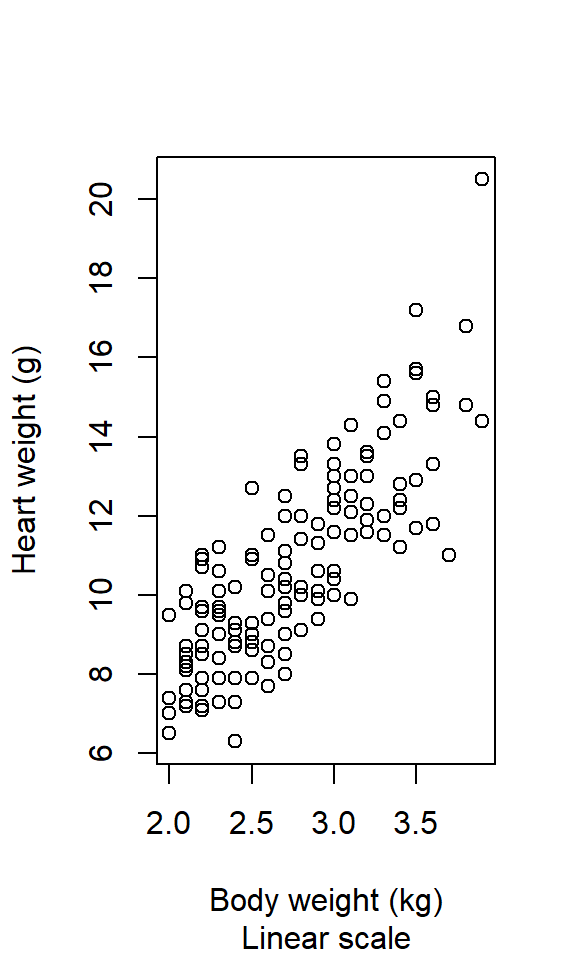
\includegraphics{20190215_files/figure-latex/unnamed-chunk-5-1.pdf}

\hypertarget{poisson-log-linear-models-in-2x2-table}{%
\section{Poisson log linear models in 2x2
table}\label{poisson-log-linear-models-in-2x2-table}}

\[\{Y_{ij}\} \sim indep.\ Poisson(\{\mu_{ij}\})\]

\begin{center}
 \begin{tabular}{|c | c | c |}
 \hline
 x&x_2=1&x_2=0\\ [0.5 ex]
 \hline
 x_1=1&$\mu_{11}$&$\mu_{12}$\\
 \hline
 x_1=0&$\mu_{21}$&$\mu_{22}$\\
 \hline
\end{tabular}
\end{center}

Row 1: \(x_1=1\), Row 2: \(x_1=0\), Column 1: \(x_2=1\), Column 2:
\(x_2=0\)

Log linear model:
\(ln(\mu_i) = \beta_0 + \beta_1 x_1 + \beta_2 x_2 + \beta_3 x_1x_2\)

Plugging in values from the table:

\begin{itemize}
\tightlist
\item
  \(ln\mu_{11} = \beta_0 + \beta_1 + \beta_2 + \beta_3\)
\item
  \(ln\mu_{12} = \beta_0 + \beta_1\)
\item
  \(ln\mu_{21} = \beta_0 + \beta_2\)
\item
  \(ln\mu_{22} = \beta_0\)
\end{itemize}

Odds ratio:
\(ln\theta = ln\mu_{11} + ln\mu_{22} - ln\mu_{12} - ln\mu_{21} = \beta_3\)


\end{document}
